\subsection{Problem najkrótszej ściezki w grafach nieważonych}
\subsubsection{Wykorzystanie DFS dla drzew}
\subsubsection{Wykorzystanie BFS dla dowolnych grafów}

\subsection{Problem najkrótszej ściezki w grafach ważonych}

W tym rozdziale poprzez \textit{spacer} będziemy rozumieli dowolny
ciąg wierzchołków $v_0$, $v_1$, $\dots$, $v_{n}$, w 
którym dla każdego $i \in \{0, 1, n-1\}$,
istnieje krawędź (może być skierowana)
$v_iv_{i+1}$. Poprzez \textit{ścieżkę}
będziemy rozumieli dowolny spacer, w którym
żadne wierzchołki nie powtarzają się.

\begin{lemma}
	Niech $(G,\omega)$ będzie skierowanym grafem ważonym 
	bez ujemnych cykli oraz niech $u,v \in V(G)$ będą
	takie, że $u \neq v$. Wtedy
	każdy spacer od $u$ do $v$ ma wagę nie 
	mniejszą niż waga
	najkrótszej ścieżki od $u$ do $v$.
	\begin{proof}
		Przypuśćmy, że istnieje taki $u$-$v$-spacer $S$, 
		którego waga jest mniejsza niż waga najkrótszej
		$u$-$v$-ściezki $P$. 
		
		Zauważmy, że spacer $S$ nie może być ścieżką, 
		bo wtedy $P$ nie jest najkrótszą ścieżką co 
		byłoby sprzeczne z doborem $P$.
		
		Skoro, $S$ nie jest ścieżką, to musi zawierać
		w sobie $k\geq 1$ cykli $C_1$, $C_2$, $\dots$, $C_k$. 
		
		Niech $Q$ to ścieżka utworzona z $S$ w taki sposób,
		że każdy cykl jest pominięty. (np. dla $S=uabcdbgv$, 
		$Q=uabgv$)
		
		Zauważmy, że
		\[\omega(P) > \omega(S) \geq \omega(Q),\]
		gdzie pierwsza nierównwność to założenie o
		tym, że $S$ jest mniejszego kosztu, a druga wynika,
		z faktu że w $G$ nie ma ujemnych cykli.
		
		Ale przecież, założyliśmy, że $P$ jest najkrótszą ścieżką,
		co prowadzi do sprzecności.
		
	\end{proof}
	\label{minpath_walk}
\end{lemma}

\begin{lemma}
	Niech $(G, w)$ będzie skierowanym grafem ważonym
	bez ujemnych cykli oraz niech $u, v \in V(G)$,
	będą takie, że $u \not = v$. Niech $P$ to 
	najkrótsza ścieżka od $u$ do $v$. Oznaczmy przez
	$x$ przedostatni wierzchołek $P$ oraz 
	przez $P'$ fragment ścieżki $P$ od $u$ do $x$.
	
	Wówczas śieżka $P'$ jest najkrótszą ścieżką od $u$ do 
	$x$.
	
	\begin{proof}
		Przypuśćmy, że tak nie jest, tzn., że istnieje 
		$u$-$x$-ścieżka $P''$, taka, że 
		$\omega(P'') < \omega(P')$ (waga ścieżki $P''$
		jest mniejsza niż waga ścieżki $P'$).
		
		Zdefiniujmy $u$-$v$-spacer $R$ jako $P'' + vx$
		(tzn. ścieżka $P''$ z krawędzią $vx$ 
		dodaną na końcu). Wtedy prawdą jest, że
		\[\omega(R) = \omega(P'') + \omega(vx) <
		\omega(P') + \omega(vx) = \omega(P),\]
		zatem udało nam się skonstruować 
		$u$-$v$-spacer $R$, który ma wagę mniejszą niż
		najmniejsza $u$-$v$-ścieżka $P$, co 
		jest sprzeczne z lematem \ref{minpath_walk}.
	\end{proof}
	\label{minpath_subpath}
\end{lemma}
\subsubsection{Algorytm Bellmana-Forda}
Algorytm Bellmana-Forda służy do znajdowania 
najkrótszej ścieżki w grafie skierowanym ważonym $(G, w)$,
\ul{nieposiadającym cykli o ujemnej długości}, przy 
\ul{dowolnych wagach krawędzi}, % może textit zamiast ul?
z wierzchołka startowego $s \in V(G)$
do dowolnego osiągalnego wierzchołka.

\begin{algorithm}[H]
	\caption{Algorytm Bellmana-Forda}\label{bellmanford_alg}
	\begin{algorithmic}[1]
		\Procedure{BellmanFord(($G, w$), $s \in V(G)$))}{}
		\State odległość = tablica liczb, rozmiaru $V[G]$
		\For{$v \in V(G)$}
		\State odległość$[v]=\infty$
		\EndFor
		\State odległość$[s]=0$
		\For{$i=1,2,\dots,n-1$}
		\For{$uv \in E(G)$}
		\If{odległość$[v] >$ odległość$[u]$ + $w(uv)$}
		\State odległość$[v]=$ odległość$[u] + w(uv)$ 
		\EndIf
		\EndFor
		\EndFor
		\State \Return odległość
		\EndProcedure
	\end{algorithmic}
	\label{bellman_ford}
\end{algorithm}
Powyższą implementację można rozbudować o
znajdowanie (i zwracanie) najkrótszych ścieżek
(algorytm \ref{Zadanie31}).

Złożoność pesymistyczna powyższego algorytmu to $O(nm)$.
Najgorsza złożoność, czyli $O(n^3)$ zajdzie dla grafów 
gęstych lub dla dowolnych grafów
zareprezentowanych z użyciem reprezentacji macierzowej, co wynika
z potrzeby przejścia po całej macierzy sąsiedztwa w pętli w linii nr. 7.

\begin{theorem}[Poprawność algorytmu Bellmana-Forda]
	Jeśli
	$(G, w)$ jest ważonym grafem skierowanym
	bez ujemnych cykli oraz
	$s \in V(G)$, to algorytm \ref{bellman_ford}
	poprawnie rozwiązuje problem najkrótszej ścieżki.
	\begin{proof}
		Dla wierzchołka $v \in V (G)$ znaczmy 
		przez $d(v)$ odległość w grafie
		$(G, w)$ od $s$ do $v$. 
		Ponadto, dla dowolnej liczby
		naturalnej $k$ i 
		wierzchołka $v \in V(G)$ niech 
		$d^{(k)}(v)$ oznacza minimalną długość 
		spaceru o co najwyżej $k$ krawędziach
		od $s$ do $v$. W przypadku kiedy $s$-$v$-spacer
		nie istnieje przyjmujemy, że $d(v), d^{(k)}(v)$
		są nieskończone.
		
		Zaczniemy od pokazania, że odległości 
		od wierzchołka $s$ 
		wyznaczane przez algorytm nigdy nie są mniejsze niż
		faktyczne odległości w $(G, w)$.
		
		\textbf{Stwierdzenie:} W każdym momencie
		działania algorytmu dla każdego wierzchołka
		$v \in V(G)$ zachodzi 
		\[\text{odległość}[v] \geq d(v).\]
		
		\textbf{Dowód stwierdzenia:} Wykorzystujemy
		indukcję matematyczną po liczbie wywołań linii nr. 9 algorytmu. 
		
		Zauważmy, że dla zerowej liczby wywołań teza jest spełniona,
		bo tablica odległości jest wypełniona nieskończonościami 
		(formalnie: liczbami większymi niż największa waga w $(G, \omega)$)
		oraz $\text{odległości}[s]=d(s)=0$, co oznacza, że
		baza indukcyjna jest spełniona.
		
		Przypuśćmy, że stwierdzenie jest prawdziwe przed pewnym
		wywołaniem lini nr. 9, co oznacza, że 
		$\text{odległość}[u] \geq d(u)$. 
		
		Korzystając z lematu 
		\ref{minpath_walk}, wiemy, że spacer składający 
		się z najkrótszej ścieżki od $s$ do $u$ z dodaną 
		na końcu krawędzią $uv$ jest nie krótszy niż 
		najkrótsza ścieżka od $s$ do $v$, co możemy 
		wyrazić jako:
		\[d(u) + \omega(uv) \geq d(v),\]
		łącząc z poprzednią nierównością otrzymujemy
		\[\text{odległość}[u] + \omega(uv) \geq d(v),\]
		co gwarantuje nam prawdziwość stwierdzenia po 
		rozważanym wykonaniu linii nr. 9. Na mocy indukcji stwierdzenie musi być prawdziwe.
		
		Z powyższego stwierdzenia wnioskujemy, że
		OPT $\leq$ REZULTAT. Wprowadźmy oznaczenie, że $\text{odległość}_i$ to 
		stan tablicy po $i$ iteracjach.
		Pokażmy prawdziowość następującego 
		niezmiennika. 
		
		\textbf{Niezmiennik:} Dla każdego 
		$i \in \{0,1, \dots, n-1\}$ po $i$ iteracjach
		pętli w linii 6 prawdą jest, że dla każdego 
		wierzchołka $v \in V(G)$ zachodzi
		\[\text{odległość}_i[v] \leq d^{(i)}(v).\]
		
		\textbf{Dowód niezmiennika:} Stosujemy indukcję
		po liczbie iteracji $i$. 
		
		Zauważmy, że skoro w grafie $G$ nie ma ujemnych 
		cykli to $d(s) = 0$, możemy zapisać, że
		\[\text{odległość}_0[s] = 0 = d(s) \leq d^{(0)}(s),\]
		co oznacza, że baza indukcji ($i=0$) jest spełniona.
		
		Przypuśćmy, że niezmiennik jest zachowany dla $i=j$,
		gdzie $j\in \{0, 1, \dots, n-2\}$, tzn., że po $j$
		iteracjach pętli w linii nr. 6 dla każdego wierzchołka
		$v$ zachodzi
		\[\text{odległość}_j[v] \leq d^{(j)}(v).\]
		
		Ustalmy dowolny wierzchołek $v$. Pokażemy, że
		$\text{odległość}_{j+1}[v] \leq d^{(j+1)}(v)$. Jeśli
		$\text{odległość}_j[v] \leq d^{(j+1)}(v)$ to koniec, 
		ponieważ wartości elementów tablicy odległość
		nie mogą się zwiększać w trakcie działania algorytmu.
		
		Przypuśćmy, że $\text{odległość}_j[v] > d^{(j+1)}(v)$.
		Niech $P$ będzie najkrótszą ścieżką od $s$ do $v$
		o nie więcej niż $j+1$ krawędziach, $x$ przedostatnim 
		wierzchołkiem $P$, a $P'$ fragmentem tej ścieżki
		zaczynającym się w $s$ i kończącym się w $x$, wtedy
		\[\omega(P) = d^{(j+1)}(v) \land \omega(P') = d^{(j)}(x),\]
		gdzie drugi fakt wynika z lematu \ref{minpath_subpath} (
		założenie o maksymalnej liczbie krawędzi nie uniewaznia
		tego lematu).
		Korzystając z założenia indukcyjnego
		\[\text{odległość}_j[x] \leq d^{(j)}(x)=\omega(P'),\]
		dodając $\omega(xv)$ obustronnie, otrzymamy
		\[\text{odległość}_j[x] + \omega(xv) \leq \omega(P') 
		+ \omega(xv) = \omega(P) = d^{(j+1)}(v).\]
		Zauważmy, że z założenia $\text{odległość}_j[v] > d^{(j+1)}(v)$,
		wynika, że warunek linii nr. 8 zostanie spełniony,
		a więc napewno wykona się linia nr. 9, czyli
		\[\text{odległość}_{j+1}[v]\leq 
		\text{odległość}_j[x] + \omega(xv),\]
		więc ostatecznie
		\[\text{odległość}_{j+1}[v]\leq d^{(j+1)}.\]
		Na mocy indukcji matematycznej niezmiennik jest prawdziwy.
		
		Z powyższego niezmiennika wnioskujemy, że 
		$\text{odległość}_{n-1}[v] \leq d^{(n-1)}(v) = d(v)$ dla dowolnego 
		$v \in V(G)$, co daje
		REZULTAT $\leq$ OPT,
		więc ostatecznie OPT $=$ REZULTAT, co kończy dowód.
		
	\end{proof}
	\label{bellmanford_proof}
\end{theorem}

\subsubsection{Algorytm Dijkstry}
Algorytm Dijkstry stanowi algernatywę do algorytmu
Bellmana-Forda, pod warunkiem, że graf wejściowy
jest grafem (skierowanym) ważonym $(G, \omega)$, 
gdzie każda krawędź ma \ul{nieujemną} wagę. 
Tak samo jak algorytm Belmmana-Forda, 
Algorytm Dijkstry znajduje wszystkie ścieżki 
do osiągalnych wierzchołków z 
wierzchołka wejściowego $s$. 

Założenie o nieujemnych wagach krawędzi pozwala na 
sformuowanie poniższego lematu.
\begin{lemma}
	Jeśli $(G, w)$ jest ważonym grafem skierowanym
	bez ujemnych wag krawędzi oraz $P = v_1v_2\dots v_k$
	jest najkrótszą ścieżką od $v_1$ do $v_k$ w $G$,
	wówczas odległość w grafie $G$ od $v_1$ do $v_{k-1}$ jest 
	nie większa niż odległość od $v_1$ do $v_k$.
	\begin{proof}
		Rozważmy pewną najkrótszą ścieżkę $P = v_1v_2
		\dots v_k$ w $G$. Na mocy lematu 
		\ref{minpath_subpath} $P'=v_1v_2 \dots v_{k-1}$
		jest najkrótszą ścieżką od $v_1$ do $v_{k-1}$.
		Zatem $\omega(P) = \omega(P') + v_1v_{k-1}$, więc
		z założenia, że wagi są nieujemne
		wynika, że  
		$\omega(P) \geq \omega(P')$. 
	\end{proof}
	\label{lemma_dijkstra}
\end{lemma}

Zauważmy, że lemat \ref{lemma_dijkstra} implikuje, że
dowolna podścieżka pewnej ścieżki $P$ musi mieć wagę
nie większą niż ścieżka $P$.

\begin{algorithm}[H]
	\caption{Algorytm Dijkstry}\label{dijkstra_alg}
	\begin{algorithmic}[1]
		\Procedure{Dijkstra(($G, \omega$), $s \in V(G)$))}{}
		\State Niech odległość to tablica liczb, rozmiaru $V[G]$
		\State Niech Q to pusta kolejka priorytetowa 
		\For{$v \in V(G)$}
		\State odległość$[v]\gets\infty$
		\EndFor
		\State odległość$[s]\gets 0$
		\State Q.Push(s, odległość[s])
		\While{Q.IsEmpty = \textit{False}}
		\State $u =$ Q.ExtractMin()
		\For{$v \in N(u)$}
		\If {$\text{odległość}[u] + \omega(uv) < 
			\text{odległość}[v]$}
		\State $\text{odległość}[v] \gets \text{odległość}[u] + \omega(uv)$
		\State Q.DecreaseKey($v$, odległość$[v]$);
		\EndIf
		\EndFor
		\EndWhile
		\State \Return odległość
		\EndProcedure
	\end{algorithmic}
	\label{dijkstra}
\end{algorithm}

Algorytm \ref{dijkstra}, tak samo jak algorytm Belmmana-Forda,
możemy rozbudować o zwracanie ścieżek.

Zakładając, że kolejka priorytetowa jest oparata na kopcach 
Fibonacciego otrzymujemy złożoność $O(n\log n + m)$. 

\begin{theorem}[Poprawność algorytmu Dijkstry]
	Jeśli $(G, \omega)$ jest ważonym grafem (skierowanym)
	bez ujemnych wag krawędzi, wówczas algorytm Dijkstry,
	dla danych $(G, \omega)$ i dowolnego $s \in V(G)$, 
	poprawnie rozwiązuje problem najkrótszej ścieżki.
	
	\begin{proof}
		Przez $d(v)$ będziemy oznaczać odległość w 
		grafie $(G, w)$
		od $s$ do $v$. Na potrzeby notacji 
		będziemy utożsamiać
		kolejkę $Q$ ze zbiorem wierzchołków, które
		się w niej znajdują (i na przykład zapis $v \in Q$ 
		będzie dla nas oznaczał, że
		wierzchołek $v$ znajduje się w kolejce).
		Poprawność algorytmu wyniknie z poniższego niezmiennika.
		
		\textbf{Niezmiennik: } Na początku oraz po 
		każdej iteracji pętli w linii nr 8 prawdziwe są 
		następujące własności:
		\begin{itemize}
			\item[(a)] Dla każdego wierzchołka $w \not \in Q$
			zachodzi odległość$[w] = d(w)$ 
			\item[(b)] Dla każdego wierzchołka $w \in Q$,
			odległość$[w]$ jest długością najkrótszej
			ścieżki od $s$ do $w$, której pierwszy wierzchołek 
			i wszystkie wierzchołki wewnętrzne nie znajdują się 
			w $Q$ 
		\end{itemize}
		\textbf{Dowód niezmiennika: } Indukcja po iteracjach
		pętli w linii nr 8.
		
		Warunki (a), (b) są spełnione przed pierwszą iteracją
		pętli, ponieważ, $Q$
		nie posiada żadnych wierzchołków poza 
		kolejką $Q$, co oznacza, że baza indukcyjna jest spełniona.
		
		Od teraz poprzez tablicę odległość będziemy rozumieli 
		stan tablicy przed wykonaniem się $i$-tej iteracji, 
		natomiast przez odległość$'$ po wykonaniu się $i$-tej iteracji.
		Tak samo $Q$ to stan kolejki przed $i$-tą iteracją,
		a $Q'$ to stan po tej iteracji. 
		
		Chcemy pokazać, że jeśli $Q$ oraz odległość spełniają
		warunki (a) i (b), to $Q'$ oraz odległosć$'$ 
		spełniają warunki (a$'$) i (b$'$).
		
		Najpierw pokażemy, że (a$'$), czyli, że
		dla każdego wierzchołka $w \not \in Q'$ zachodzi
		odległość$'[w] = d(w)$. Niech $u$ to wierzchołek
		zdjęty z kolejki priorytetwowej w linijce nr. 9.
		Zauważmy, że odległość$'[u] = \text{odległość}[u]$. 
		Aby wykazać prawdziwość tego warunku wystarczy
		pokazać, że $\text{odległość}[u] = d(u)$, ponieważ
		$u$ to jedyny wierzchołek, który został zdjęty z kolejki
		(wszystkie pozostałe wierzchołki spełniają 
		(a$'$) na mocy (a)).
		
		Przypuśćmy, że istnieje 
		$s$-$u$-ścieżka $P$ taka, że $\omega(P) < \text{odległość}[u]$. 
		Z (b) wynika, że odległość$[u]$ jest odległością 
		najmniejszej ścieżki wzdłuż wierzchołków z poza $Q$, co
		oznacza, że $P$ musi mieć co najmniej jeden wierzchołek 
		w $Q$, który nie jest wierzchołkiem $u$. 
		Oznaczmy pierwszy wierzchołek z $Q$ na ścieżce $P$ jako $x$. 
		
		Z (b) wynika, że $\omega(sPx) = \text{odległość}[x]$, natomiast
		z warunku kolejki, wiemy, że
		$\text{odległość}[x] \geq \text{odległość}[u]$. Aby 
		warunek $\omega(P) < \text{odległość}[u]$ był spełniony
		w $(G, \omega)$ musiałyby istnieć krawędzie 
		z ujemnymi wagami (z lematu \ref{lemma_dijkstra} implikujemy, że
		dowolna podścieżka $P$ o początku w $s$
		musi mieć nie większą wagę niż ścieżka $P$) co jest sprzeczne z założeniem, czyli
		$\text{odległość}[u] = d(v)$
		co oznacza, że (a$'$) jest spełnione.
		
		Teraz pokażemy, że (b$'$), czyli, że
		dla każdego wierzchołka $w \in Q'$, 
		$\text{odległość}'[w]$ jest równa minimalnej długości
		ścieżki z $s$ do $w$, której pierwszy wierzchołek i 
		wszystkie wierzchołki wewnętrzne 
		nie znajdują się w $Q'$. Ponownie 
		przez $u$ oznaczamy wierzchołek
		zdjęty z kolejki priorytetwowej w linijce nr. 9.
		
		Z przebiegu pętli, możemy wyodrębnić następujące 
		przypadki: 
		\begin{itemize}
			\item[1.] $w \not \in N(u) \Rightarrow$ 
			odległość$'[w]=$ odległość$[w]$, a więc (b) 
			implikuje (b'), bo nie powstaje żadna nowa ścieżka, 
			której pierwszy wierzchołek i wszystkie wierzchołki
			wewnętrzne nie znajdują się w $Q$
			\item[2.] $w \in N(u) \Rightarrow$ 
			powstaje dokładnie jedna nowa ścieżka $P$, 
			której pierwszy wierzchołek i wszystkie wierzchołki
			wewnętrzne nie znajdują się w $Q$. Z (a$'$) wynika, że
			odległość$'[u] = d(u)$, więc 
			\[\omega(P) = d(u) + \omega(uw) = \text{odległość}'[u] + \omega(uw) = \text{odległość}[u] + \omega(uw).\]
			
			Algorytm w linijce nr 11. dokonuje porównania, które 
			skutkuje zapisaniem $\omega(P)$, w przypadku
			kiedy możliwe jest poprawienie odległości dla $w$. Z faktu, że
			$P$ to jedyna taka ścieżka, która może poprawić odległość
			implikujemy, że (b$'$) jest spełnione
		\end{itemize}
		
		
		
		Na mocy indukcji matematycznej niezmiennik musi być prawdziwy.
		
		Zauważmy, że po ostatniej iteracji głównej pętli kolejka $Q$ musi być pusta,
		zatem część (a) niezmiennika pociąga za sobą
		poprawność algorytmu.
	\end{proof}
	\label{dijkstra_proof}
\end{theorem}


\subsubsection{Algorytm A\texorpdfstring{$^*$}{TEXT}}
Algorytm A$^*$ działa w sposób analogiczny do algoyrtmu Dijkstry, 
ale służy do znajdywania ścieżki pomiędzy dwoma zadanymi wierzchołkami
$s$ i $t$, a nie jak w przypadku algorytmu Dijkstry pomiędzy $s$
i wszystkimi innymi wierzchołkami w grafie.

Algorytm A$^*$ wykorzysuje heurystykę $h$ (jedna z wartości 
wejściowych), gdzie dla wierzchołka
$v \in G$, $h(v)$ definiujemy jako oszacowanie
na odległość od $v$ do $t$. Założenia danych wejściowych są następujące
\begin{itemize}
	\item nieujemne wagi krawędzi,
	\item dla każdego wierzchołka $v$ zachodzi $h(v) \leq \text{dist}(v, t)$,
	\item dla każdej krawędzi $uv$ zachodzi $h(u) \leq h(v) + \omega(uv)$ (warunek zgodności).
\end{itemize}
Dla grafu, którego wierzchołkami są miasta na mapie, a wagami krawędzi odległości drogowe, przykładem heurystyki spełniającej powyższe założenia jest odległość miast w linii prostej.

 Ideą algorytmu jest przeszukiwanie wierzchołków $v$ w kolejności 
rosnącego $\text{dist}(s,v) + h(v)$. 

\begin{algorithm}[H]
	\caption{Algorytm A*}
	\begin{algorithmic}[1]
		\Procedure{AStar($(G, \omega)$, $s$, $t$, $h$)}{}
		\State Niech odległość to tablica liczb, rozmiaru $V[G]$
		\For{$v \in V(G)$}
		\State odległość$[v]\gets\infty$
		\EndFor
		\State odległość$[s]\gets 0$
		\State Q - kolejka priorytetowa inicjalizowana 
		zbiorem $\{V(G)\}$, gdzie priorytet każdego wierzchołka $v$
		to odległość$[v] + h(v)$
		\While{Q.IsEmpty = \textit{False}}
		\State $u =$ Q.ExtractMin()
		\If{u = t}
		\State \textit{break}
		\EndIf
		\For{$v \in N(u)$}
		\If {$\text{odległość}[u] + \omega(uv) < 
			\text{odległość}[v]$}
		\State $\text{odległość}[v] \gets \text{odległość}[u] + \omega(uv)$
		\State Q.DecreaseKey($v$, odległość$[v] + h(v)$)
		\EndIf
		\EndFor
		\EndWhile
		\State \Return odległość$[t]$
		\EndProcedure
	\end{algorithmic}
	\label{aStar_alg}
\end{algorithm}

Zauważmy, że w przypadku kiedy $h(v) = 0$ dla każdego $v \in G$ 
to algorytm A$^*$ jest równoważny algorytmowi Dijkstry, co oznacza, że
złożoność pesymistyczna tego algorytmu jest taka sama jak złożoność
pesymistyczna algorytmu Dijsktry.

Okazuje się, że przy dobrej heurystyce, mamy szansę na 
przeszukanie $o(n)$ wierzchołków. Przebieg konstruowania
dobrej heurystyki, zależy od problemu z którym się mierzymy. 
Przykładowo, wyobraźmy sobie, że szukamy odległości z miasta $A$
do miasta $B$ na mapie samochodowej. Każde połączenie jakąś drogą
jest krawędzią z wagą oznaczającą liczbę kilometrów, natomiast
każde miasto to wierzchołek grafu. Jako heurystykę w tym problemie 
możemy przyjąć odległość euklidesową od każdego miasta
do miasta docelowego, jako że droga pomiędzy miastami nie może mieć 
mniejszej długości niż odległość euklidesowa, oba warunki
heurystyki są spełnione.

\begin{theorem}
	[Poprawność algorytmu A$^*$] Jeśli
	$(G, w)$ jest ważonym grafem skierowanym
	z wagami nieujemnymi,
	$s,t \in V(G)$, oraz heurystyka $h(v)$
	spełnia następujące założenia:
	\begin{itemize}
		\item dla każdego wierzchołka $v$ zachodzi $h(v) \leq \text{dist}(v, t)$,
		\item dla każdej krawędzi $uv$ zachodzi $h(u) \leq h(v) + \omega(uv)$,
	\end{itemize}
	to algorytm \ref{aStar_alg}
	poprawnie rozwiązuje problem najkrótszej ścieżki
	pomiędzy wierzchołkami $s$ i $t$.
	\begin{proof}
		\textbf{to do} (nie obowiązuje na kolokwium)
	\end{proof}
	\label{aStar_proof}
\end{theorem}

\subsubsection{Algorytm Johnsona}
Algorytmy Johnsona jak i Floyda-Warshalla 
różnią się od poprzedników tym, że
ścieżki znajdowane są pomiędzy każdą parą
wierzchołków z tego grafu.

Algorytm Johnsona opiera się na sprytnym wykorzystaniu
algorytmu Bellmana-Forda oraz algorytmu Dijkstry. Na 
wejściu przyjmowane są grafy (skierowane) o dowolnych
wagach, bez cyklów o ujemnej długości. Ideą tego
algorytmu jest skonstruowanie równoważnego 
grafu o nieujemnych wagach na krawędziach,
w celu zastosowania algorytmu Dijsktry.

W tym miejscu warto zaznaczyć, że skonstruowanie takiego
grafu nie może odbyć się przez zwyczajne dodanie
do wagi każdej krawędzi, wartości $|\!\min_{v \in V(G)}{\omega(v)}|$. 
Rysunek \ref{fig:kontrprzyklad_johnson}
przedstawia kontrprzykład -- w grafie wejściowym
optymalna $s$-$u$-ścieżka to $svwu$, natomiast
w grafie wyjściowym, otrzymanym po dodaniu
$|\!\min_{v \in V(G)}{\omega(v)}| = 15$ do każdej 
wagi, optymalną $s$-$u$-ścieżką jest $su$.

\begin{figure}[H]
	\centering
	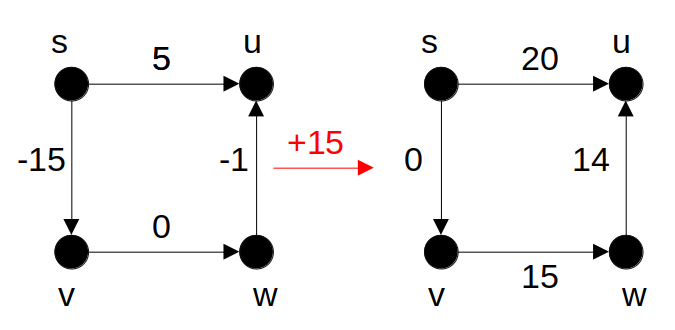
\includegraphics[width=0.4\textwidth]{data/graf_rownowazny_kontrprzyklad.png}
	\caption{  }
	\label{fig:kontrprzyklad_johnson}
\end{figure}

Konstrukcja grafu równoważnego $(G', \omega')$ 
do grafu wejściowego $(G, \omega)$
w algorytmie Johnsona polega na
dodaniu do $G$ wierzchołka $q$, oraz 
dla każdego wierzchołka $v \in V(G)$ krawędzi
skierowanych $qv$ z wagą 0. 

W następnym kroku wywołujemy algorytm Belmmana-Forda
na grafie $(G', \omega')$ z wierzchołkiem 
startowym $q$, po to aby utworzyć nową funkcję wagową,
na $G$, która zawsze będzie przyjmować wartości 
nieujemne, co umożliwi zastowanie 
algorytmu Dijsktry. 

\begin{algorithm}[H]
	\caption{Algorytm Johnsona}
	\begin{algorithmic}[1]
		\Procedure{Johnson($G, \omega$)}{}
		\State Niech $V'=V(G) \cup \{q\}$ oraz 
		$E' = E(G) \cup \{qv : v \in V(G)\}$
		\State Skonstruuj graf skierowany $(G', V')$
		\State Zdefiniuj funkcję $\omega' : E' \to \mathbb{R}$, 
		gdzie 
		\[\omega'(e) = \begin{cases}
			\omega(e), \text{ jeśli } e \in E(G) \\
			0, \text{ jeśli }  e \not \in E(G)   
		\end{cases}\]
		\State $h = \text{BellmanFord}((G', \omega'), q)$
		\State Zdefiniuj funkcję $\omega'' : E(G) \to \mathbb{R}$, 
		gdzie 
		\[\omega''(uv) = \omega(uv) + h(u) - h(v)\]
		\For{$u \in V(G)$}
		\State $d_u = \text{Dijsktra}((G, \omega''), u)$
		\For{$v \in V$}
		\State odległości$[u, v] = d_u[v] - h[u] + h[v]$
		\EndFor
		\EndFor
		\State \Return odległości
		\EndProcedure
	\end{algorithmic}
	\label{Johnson}
\end{algorithm}

Zakładając, że kolejka priorytetowa zastosowana 
w algorytmie Dijsktry jest oparata na kopcach 
Fibonacciego otrzymujemy złożoność $O(n^2\log n + nm)$. Algorytm 
ten jest szybszy niż później omawiany 
algorytm Floyda-Warshalla, dla graów rzadkich. 

\begin{theorem}[Poprawność algorytmu Johnsona]
	Jeśli $(G, \omega)$ jest ważonym grafem skierowanym
	bez ujemnych cykli, to algorytm Johnsona dla 
	danych wejściowych $(G, \omega)$ poprawnie
	rozwiązuje problem najkrótszej ścieżki 
	pomiędzy dowolnymi parami wierzchołków.
	
	\begin{proof}
		Przez $dist_\chi(u, v)$ oznaczmy wagę minimalnej ścieżki
		z wierzchołka $u$ do $v$ przy ważeniu $\chi$ domyślając się, 
		że chodzi o graf $G$ lub $G'$ w zależności od dziedziny $\chi$.
		% niezrozumiałe XD
		
		Aby wykazać poprawność aglorytmu Johnsona 
		musimy udowodnić poniższe obserwacje:
		\begin{itemize}
			\item[1. ] Dane wejściowe do 
			algorytmu Bellmana-Forda są poprawne.
			\item[2. ] Dane wejściowe do 
			algorytmu Dijkstry są poprawne.
			\item[3. ] Niech $P$ to dowolna
			$u$-$v$-ścieżka w grafie $G$ oraz niech $h$
			to odwzorowanie zwrócone przez algorytm
			Belmmana-Forda w linii nr. 5, wtedy
			\[\omega''(P) = \omega(P) +  h(u) - h(v).\]
			\item[4. ] Niech $u, v \in V(G)$, wtedy
			\[dist_{\omega}(u, v) = dist_{\omega''}(u, v) - h(u) + h(v).\]
		\end{itemize}
		
		Obserwacja 1. jest prawdziwa, ponieważ ($G$, $\omega$)
		z założenia nie posiada ujemnych cykli oraz
		dodanie do $G$ wierczhołka $q$ z krawędziami skierowanymi
		od $q$ do każdego wierzchołka z $G$ nie może utworzyć
		żadnego nowego cyklu, a więc w szczególności nie może
		w ten sposób powstać żaden ujemny cykl, co oznacza, że
		$(G', \omega')$ oraz $q$ to poprawne dane wejściowe
		do algorytmu Bellmana-Forda.
		
		\textbf{Dowód obserwacji 2:} Niech $uv \in E(G')$, 
		wtedy prawdą jest, że
		\[dist_{\omega'}(q, v) \leq dist_{\omega'}(q, u) + \omega'(uv),\]
		co w połączeniu z poprawnością algorytmu Belmmana-Forda (tw.
		\ref{bellmanford_proof}) oraz faktem, że 
		$uv \in E(G)$ daje nam
		\[h(v) \leq h(u) + \omega(uv).\]
		Po przeniesieniu $h(v)$ na prawą stronę otrzymujemy 
		\[0 \leq \omega(uv) + h(u) - h(v) = \omega''(uv),\]
		więc każda krawędź grafu ważonego $(G, \omega'')$ ma
		nieujemną wagę, co oznacza, że wywołanie algorytmu 
		Dijkstry jest poprawne.  
		
		\textbf{Dowód obserwacji 3:} Niech $P=v_1v_2\dots v_k$, 
		gdzie $v1 = u$ oraz $v_k = v$ to dowolna $u$-$v$-ścieżka
		w grafie $G$, wtedy 
		\[\omega''(P) = \omega''(v_1v_2) + \omega''(v_2v_3) + \dots + \omega''(v_{k-1}v_k),\]
		korzystając z definicji $\omega''$ otrzymamy
		\[\omega''(P) = \omega(v_1v_2) + h(v_1) - (h_2) + 
		\omega(v_2v_3) + h(v_2) - (h_3) + 
		\dots + \omega(v_{k-1}v_k) + h(v_{k-1}) - (h_k),\]
		po uporządkowaniu powyższego dostaniemy
		\[\omega''(P) = \omega(P) + \omega(v_1) - \omega(v_k) = \omega(P) + h(u) - h(v),\]
		co należało dowieść.
		
		\textbf{Dowód obserwacji 4:} Niech $P_{\omega}$ oraz 
		$P_{\omega''}$ to najkrótsze $u$-$v$-ścieżki kolejno 
		przy ważeniu $\omega$ oraz $\omega''$. Korzystając z 
		Obserwacji 3 otrzymujemy
		\[\omega''(P_{\omega}) = \omega(P_{\omega}) + h(u) - h(v) \leq
		\omega(P_{\omega''}) + h(u) - h(v) = \omega''(P_{\omega''}),\]
		co wynika, z założenia, że $P_{\omega}$ to 
		najmniejsza ścieżka w $(G, \omega)$. 
		
		Z powyższej nierówności oraz z założenia, że $P_{\omega''}$ to 
		najmniejsza ścieżka w $(G, \omega'')$ otrzymujemy
		\[\omega''(P_{\omega''}) \leq \omega''(P_{\omega}) \leq \omega''(P_{\omega''}), \]
		\[\omega''(P_{\omega''}) = \omega''(P_{\omega}),\]
		a zatem po ponownym zastosowaniu obserwacji 3
		\[\omega''(P_{\omega''}) = \omega(P_{\omega}) + h(u) - h(v),\]
		\[\omega(P_{\omega''}) = \omega''(P_{\omega''}) - h(u) + h(v),\]
		co dzięki poprawności algorytmu Dijkstry (tw. \ref{dijkstra_proof}),
		daje nam
		\[dist_{\omega}(u, v) = dist_{\omega''}(u, v) - h(u) + h(v).\]
		
		Obserwacje 1, 2 i 4 implikują, że tablica odległości zostanie
		wypełniona poprawnie. Jako że algorytm na pewno zakończy pracę,
		dowód poprawności jest kompletny.
	\end{proof} 
\end{theorem}

\subsubsection{Algorytm Floyda-Warshalla}
\begin{algorithm}[H]
	\caption{Algorytm Floyda-Warshalla}
	\begin{algorithmic}[1]
		\Procedure{FloydWarshall($G, \omega$)}{}
		\State Utwórz tablicę odległości o wymiarach $V(G) \times V(G)$
		\For{$i \in V(G)$}
		\For{$j \in V(G)$}
		\If{$ij \in E(G)$}
		\State $\text{odległości}[i, j] = \omega(ij)$
		\Else
		\State $\text{odległości}[i, j] = \infty$
		\EndIf
		\EndFor
		\EndFor
		\For{$i \in V(G)$}
		\State $\text{odległości}[i, i] = 0$
		\EndFor
		\For{$k \in V(G)$}
		\For{$i \in V(G)$}
		\For{$j \in V(G)$}
		\If{$\text{odległości}[i, j] > \text{odległości}[i, k] + \text{odległości}[k, j]$}
		\State $\text{odległości}[i, j] = \text{odległości}[i, k] + \text{odległości}[k, j]$
		\EndIf
		\EndFor
		\EndFor
		\EndFor
		\State \Return odległości
		\EndProcedure
	\end{algorithmic}
	\label{floydWarshall_alg}
\end{algorithm}

Złożoność powyższego algorytmu to $O(n^3)$.

\begin{theorem}[Poprawność algorytmu Floyda-Warshalla]
	Jeśli $(G, \omega)$ jest ważonym grafem skierowanym
	bez ujemnych cykli, to algorytm Floyda-Warshalla dla 
	danych wejściowych $(G, \omega)$ poprawnie
	rozwiązuje problem najkrótszej ścieżki 
	pomiędzy dowolnymi parami wierzchołków.
	
	\begin{proof}
		Oznaczmy przez $d^{(m)}$(i, j) długość najkrótszej
		$i$-$j$-ścieżki, której wewnętrzne wierzchołki 
		należą do zbioru $\{0, 1, 2, \dots, m-1\}$. 
		Ponadto, przez
		$\text{odległości}_{m}[i, j]$ będziemy rozumieli 
		stan tablicy po 
		wykonaniu się $m$-tej iteracji.
		
		\textbf{Niezmiennik:} Po $l$ iteracjach 
		pętli for w linii nr. 11, dla każdych wierzchołków
		$i, j \in V(G)$ zachodzi odległości$[i,j] \leq d^{(l)}(i,j)$.
		
		\textbf{Dowód niezmiennika:} Indukcja po liczbie iteracji $l$.
		
		Wartości początkowe spełniają warunek, zatem
		baza indukcyjna jest prawdziwa. 
		
		Przypuśćmy, że $\text{odległości}_{l}[i, j] \leq
		d^{(l)}(i, j)$, chcemy pokazać, że 
		$\text{odległości}_{l+1}[i, j] \leq$$ d^{(l+1)}(i, j)$.
		W przypadku kiedy $d^{(l)}(i,j) =$$ d^{(l+1)}(i,j)$, to
		\[d^{(l+1)}(i,j) = d^{(l)}(i, j) \geq 
		\text{odległości}_l[i, j] \geq \text{odległości}_{l+1}[i, j],\]
		gdzie pierwsza nierówność wynika z założenia indukcyjnego, natomiast
		druga z 14 i 15 linii algorytmu, które implikują, że
		w każdej iteracji odległości mogą się tylko zmniejszyć lub
		nie uledz żadnej zmianie.
		
		Rozważmy przypadek, kiedy $d^{(l)}(i,j) >$$ d^{(l+1)}(i,j)$. 
		W takiej sytuacji musiała powstać co najmniej jedna 
		$i$-$j$-ścieżka. Każda z nowopowstałych $i$-$j$-ścieżek
		musi zawierać w sobie wierzchołek $l$, niech 
		$P$ to najkrótsza z nich. Zauważmy, że
		\[\omega(P) = d^{(l+1)}(i, j) = 
		d^{(l+1)}(i, l) + d^{(l+1)}(l, j),\]
		gdzie druga równość wynika z wielokrotnego zastosowania 
		lematu \ref{minpath_subpath}.
		
		Ponadto, możemy zauważyć, że $d^{(l+1)}(i, l) = d^{(l)}(i, l)$ 
		oraz $d^{(l+1)}(l, j) = d^{(l)}(l, j)$, co wynika z fatku, że
		najkrótsza ścieżka, której wnętrze składa się z wierzchołków 
		$\{0, 1, 2, \dots, l-1\}$, zaczynająca się w $l$ 
		nie być gorsza niż najkrótsza ścieżka której 
		wnętrze składa się z wierzchołków 
		$\{0, 1, 2, \dots, l-1, l\}$.
		
		Zatem ostatecznie:
		\[\text{odległości}_{l+1}[i,j] \leq 
		\text{odległości}_{l}[i,l] + \text{odległości}_{l}[l,j] \leq
		\]
		\[\leq d^{(l)}(i, l) + d^{(l)}(l, j) = d^{(l+1)}(i, l) + d^{(l+1)}(l, j) = d^{(l+1)}(i, j),\]
		gdzie pierwsza nierówność wynika z 14 oraz 15 linii algorytmu,
		natomiast druga - z założenia indukcyjnego.
		
		Na mocy indukcji matematycznej niezmiennik jest prawdziwy.
		
		\textbf{Stwierdzenie:} W każdym momencie działania algorytmu
		dla każdego wierzchołka $v \in V(G)$ zachodzi 
		\[\text{odległość}[v] \geq d(v).\]
		
		\textbf{Dowód stwierdzenia:} Indukcja po liczbie iteracji $l$.
		
		Dla zerowej liczby wywołań teza jest spełniona, a 
		zatem baza indukcyjna jest prawdziwa.
		
		Przyjmijmy, że jeśli $\text{odległości}_l[i, j] \geq d(i, j)$
		jest prawdą to $\text{odległości}_{l+1}[i, j] \geq d(i, j)$
		również musi być prawdziwe.
		
		Jeśli $\text{odległość}_{l+1}[i, j] = \text{odległość}_{l}[i, j]$,
		to korzystając z założenia indukcyjnego możemy zakończyć dowód.
		
		Rozważmy przypadek, kiedy 
		$\text{odległość}_{l+1}[i, j] < \text{odległość}_{l}[i, j]$. 
		Aby ten przypadek zaszedł musiały wykonać się linijki 14 i 15
		co oznacza, że 
		\[\text{odległość}_{l+1}[i, j] = \text{odległość}_{l}[i, l+1] 
		+ \text{odległość}_{l}[l+1, j] \geq d(i, l+1) + d(l+1, j)
		\geq d(i, j),\]
		gdzie pierwsza nierówność wynika, z założenia indukcyjnego,
		natomiast druga - z faktu, że $d(i, j)$ oznacza
		długość najkrótszej ścieżki.
		
		Na mocy indukcji matematycznej, stwierdzenie jest prawdziwe.
		
		Stwierdzenie oraz niezmiennik implikują, że 
		dla każdej pary wierzchołków
		$i, j \in V(G)$ prawdą jest, że 
		\[\text{odległość}_n[i,j] \leq d^{(n)}(i, j) = d(i, j) \leq \text{odległość}_n[i,j],\]
		a zatem
		\[\text{odległość}_n[i,j] = d(i, j),\]
		co kończy dowód.
		
	\end{proof} 
	\label{floydWarshall_proof}
\end{theorem}

\subsubsection{Podsumowanie}